\documentclass[]{article}

\usepackage[italian]{babel}
\usepackage[margin=20mm, footskip = 20pt]{geometry}
\usepackage{array}
\usepackage{tabularx}
\usepackage{graphicx}
\usepackage{subfiles}
\usepackage{hyperref}
\usepackage{nameref}
\usepackage{titlesec}
\usepackage{longtable}
\usepackage[table]{xcolor}
\usepackage{titling}
\usepackage{lastpage}
\usepackage{ifthen}
\usepackage{calc}
\usepackage{soulutf8}
\usepackage{contour}
\usepackage{float}
\usepackage{fancyhdr}
\usepackage{multirow}
\usepackage{pgfgantt}
\usepackage{lscape}

\newcommand{\hr}{\par\vspace{-.1\ht\strutbox}\noindent\hrulefill\par}

\graphicspath{ {./}
	{./commons/res}
}

%--------------------------------------------------
% Comandi per inserire contenuto del documento
%--------------------------------------------------
\makeatletter

\newcommand\appendToGraphicsPath[1]{%
	\g@addto@macro\Ginput@path{{#1}}%
}

\newcommand{\setTitle}[1]{%
	\newcommand{\@phTitle}{#1}%
}
\newcommand{\phTitle}{\@phTitle}

\newcommand{\setDate}[1]{%
	\newcommand{\@phDate}{#1}%
}
\newcommand{\phDate}{\@phDate}

\newcommand{\setUso}[1]{%
	\newcommand{\@uso}{#1}%
}
\newcommand{\uso}{\@uso}

\newcommand{\setVersione}[1]{%
	\newcommand{\@versione}{#1}%
}
\newcommand{\versione}{\@versione}

\newcommand{\disabilitaVersione}{%
	\renewcommand{\setVersione}[1]{}%
	\renewcommand{\versione}{DISABILITATA}
}

\newcommand{\setResponsabile}[1]{%
	\newcommand{\@responsabile}{#1}%
}
\newcommand{\responsabile}{\@responsabile}

\newcommand{\setRedattori}[1]{%
	\newcommand{\@redattori}{#1}%
}
\newcommand{\redattori}{\@redattori}

\newcommand{\setVerificatori}[1]{%
	\newcommand{\@verificatori}{#1}%
}
\newcommand{\verificatori}{\@verificatori}

\newcommand{\setModifiche}[1]{%
	\newcommand{\@modifiche}{#1}%
}
\newcommand{\modifiche}{\@modifiche}

\makeatother 

%--------------------------------------------------
% Comandi per i documenti esterni e il glossario
%--------------------------------------------------

\newcommand{\dext}[1]{\textsc{#1\textsubscript{\textit{D}}}}

\newcommand{\glock}[1]{\textsc{#1\textsubscript{\textit{G}}}}

%--------------------------------------------------
% Comandi per impostare sottotitoli di quarto e quinto livello
%--------------------------------------------------

\setcounter{secnumdepth}{4}
\setcounter{tocdepth}{4}

\titleformat{\paragraph}
{\normalfont\normalsize\bfseries}{\theparagraph}{1em}{}
\titlespacing*{\paragraph}{0pt}{2.25ex plus 1ex minus .2ex}{1.5ex plus .2ex}

\titleformat{\subparagraph}
{\normalfont\normalsize\bfseries}{\thesubparagraph}{1em}{}
\titlespacing*{\subparagraph}{0pt}{1.75ex plus 1ex minus .2ex}{.75ex plus .1ex}

\appendToGraphicsPath{../../../commons/res/}

%------------------------------
%
% COMANDI DI CONFIGURAZIONE
%
%------------------------------

\setTitle{Verbale esterno \#1}

\setVersione{1.0.0}

\setDate{14-12-2020}

\setResponsabile{Paolo Scanferlato}

\setRedattori{Lucia Fenu}

\setVerificatori{Alessandro Chimetto}

\setUso{Esterno}

\setModifiche{
    1.0.0 & Alessandro Chimetto & Verificatore & 16-12-2020 & Verifica stesura iniziale\\
	1.0.0 & Lucia Fenu & Redattore & 15-12-2020 & Stesura iniziale}

\begin{document}

	% Direttive per la creazione del titolo tramite comando maketitle
\title{\huge \textsc{\phTitle{}} \\
	\vspace{11pt} \large \textsc{\phDate{}}}

\author{} % Non toccare
\date{} % Non toccare

%--------------------
% Frontespizio
%--------------------

% Logo del gruppo
\begin{figure}[t!]
	\centering
	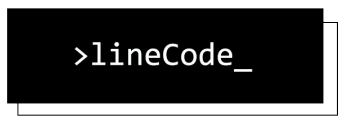
\includegraphics[width=20em]{lclong}
\end{figure}

% Titolo / Nome
\maketitle
\thispagestyle{empty}

% Dati specifici sul doc in forma tabulare
\begin{table}[ht]
	\begin{center}
		\label{tab:Dati sul documento}
		\begin{tabular}{r|l}
			\multicolumn{2}{c}{ \textsc{Dati sul documento} } \\
			\hline
			\textbf{Versione} & \versione{} \\
			\textbf{Uso} & \uso{}  \\
			\textbf{Redattori} & \redattori{} \\
			\textbf{Verificatori} & \verificatori{} \\
			\textbf{Responsabile} & \responsabile{} \\
			\textbf{Destinatari} & lineCode \\
								& prof.\ Vardanega Tullio \\		
								& prof.\ Cardin Riccardo \\
			\ifthenelse{\equal{\uso}{Esterno}}{
								& Sanmarco Informatica
			}{} \\
		\end{tabular}
	\end{center}
\end{table}

\newpage

\renewcommand{\arraystretch}{2} % allarga le righe con dello spazio sotto e sopra
\begin{longtable}[H]{>{\centering\bfseries}m{2cm} >{\centering}m{3.5cm} >{\centering}m{2.5cm} >{\centering}m{3cm} >{\centering\arraybackslash}m{5cm}}
	\rowcolor{lightgray}
	{\textbf{Versione}} & {\textbf{Nominativo}} & {\textbf{Ruolo}} & {\textbf{Data}} & {\textbf{Descrizione}}  \\
	\endfirsthead%
	\rowcolor{lightgray}
	{\textbf{Versione}} & {\textbf{Nominativo}}  & {\textbf{Ruolo}} & {\textbf{Data}} & {\textbf{Descrizione}}  \\
	\endhead%
	\modifiche{}%
\end{longtable}
	\newpage

	%--------------------------------
	%
	% IL CONTENUTO INIZIA DA QUI
	%
	%--------------------------------

	\section{Introduzione}
		\subsection{Luogo e data dell'incontro}
		\begin{itemize}
			\item \textbf{Modalità}: Telematica;
			\item \textbf{Software utilizzato}: Google Meet;
			\item \textbf{Data}: 14 Dicembre 2020;
			\item \textbf{Ora di inizio}: 16:00;
			\item \textbf{Ora di fine}: 16:45;
		\end{itemize}

		\subsection{Presenze}
		\begin{itemize}
			\item \textbf{Presenti}:
			\begin{itemize}
				\item Matteo Alba
				\item Giacomo Bulbarelli
				\item Alessandro Chimetto
				\item Alessandro Dindinelli
				\item Lucia Fenu
				\item Paolo Scanferlato
				\item Valton Tahiraj
			\end{itemize}
			\item \textbf{Assenti}:
			\begin{itemize}
				\item Nessuno
			\end{itemize}
			\item \textbf{Partecipanti esterni}:
			\begin{itemize}
			\item Alex Beggiato (referente, SanMarco Informatica)
		\end{itemize}
		\end{itemize}


		\subsection{Ordine del giorno}
		\begin{enumerate}
			\item Tecnologie consigliate;
			\item entità esterne al sistema;
			\item emplementazione guida semi-automatica;
			\item le collisioni;
			\item applicazioni \glock{real-time};
			\item disponibiltà nell'approffondire lo studio.
		\end{enumerate}

	\newpage

	\section{Svolgimento}
		\subsection{Tecnologie consigliate}
	Il committente lascia libera scelta sulle tecnologie da utilizzare a patto che sia motivata. Alcuni esempi e consigli:
	\begin{itemize}
		\item per il motore di calcolo, sviluppabile con la gestione a più \glock{thread} è possibile utilizzare:
		\begin{itemize}
			\item \bfseries{\glock{Java}};
		\end{itemize}
		\item dal punto di vista del  monitor real time, un applicativo puramente web che eventualmente dialoghi tramite web service con il motore scelto o che rielabori i dati; ad esempio:
		\begin{itemize}
			\item \bfseries{\glock{AngularJS}}:
			\item \bfseries{\glock{Angular 2+}};
			\item \bfseries{\glock{React}};
			\item \bfseries{\glock{PHP}};
		\end{itemize}
		\item 	per i simulatori di entità che girano e inviano segnali, essendo mono \glock{thread}, si può scendere su linguaggi come:
		\begin{itemize}
			\item \bfseries{\glock{Node.js}};
			\item \bfseries{\glock{Java}};
		\end{itemize}
		\item 	un uso di linguaggi compilati come \glock{C} e \glock{C++}, meglio se effettuato all'interno del motore di calcolo per motivi di performance.
	\end{itemize}

		\subsection{Entità esterne al sistema}
		Tutto ciò che è esterno al sistema e che si muove in modo casuale, non prevedibile, è riconducibile al caso dei pedoni.

		\subsection{Implementazione guida semi-automatica}
		La guida semi-automatica, come quella autonoma, prevede l'uso (base) di quattro frecce direzionali ed un pulsante start-and-stop.
		Nel primo caso, in particolare, è prevista una doppia interfaccia:
		\begin{itemize}
			\item del sistema: il consiglio che il sistema offre al guidatore in riferimento ai calcoli di percorso con ostacoli;
			\item del guidatore: la direzione che deciderà di intraprendere sulla base del consiglio di sistema e che verrà eseguita.
		\end{itemize}


		\subsection{Collisioni}
		Nel caso di una guida semi-automatica, Il sistema non avrà mai il totale controllo del veicolo.\\
		Nel caso di una possibile collisione, il sistema consiglierà sempre il guidatore senza interferire con la reale decisione di quest'ultimo. \\
		Al contrario, in un sistema autonomo come i robot, questo avrà totale controllo sulla strada da percorrere poiché sprovvisto di un guidatore.

		\subsection{\glock{Applicazioni real-time}}
		Prima di tutto è importante definire il contesto in cui verrà applicato il sistema.\\
		Infatti i tempi di risposta variano in base all'ambiente considerato, ad esempio: in un magazzino i tempi di risposta saranno più lunghi
		rispetto a quelli richiesti su strada, in cui i veicoli hanno velocità maggiore e dunque un tempo di risposta quasi immediato.

		\subsection{Disponibiltà nell'approffondire lo studio.}
		Il committente dà disponibilità per:
		\begin{itemize}
			\item \bfseries{\glock{JavaScript}};
			\item \bfseries{\glock{Canva}};
			\item \bfseries{\glock{Angular}}.
		\end{itemize}

\end{document}

